% THIS TEMPLATE IS A WORK IN PROGRESS

\documentclass[polish, a4paper]{article}
\usepackage[a4paper,left=3cm,right=3cm,top=3cm,bottom=1.5cm]{geometry}
\usepackage[T1]{fontenc}
\usepackage[polish]{babel}
\usepackage[utf8]{inputenc}
\usepackage{hyperref}
\usepackage{fancyhdr}
\usepackage{float}
\usepackage{graphicx}
\usepackage{titling}
\usepackage{wasysym}
\usepackage{caption}
\usepackage{pgfplots}
\usepackage{pgfplotstable}
\usepackage{filecontents}
\usepackage{csvsimple}
\usepackage{textcomp}
\usepackage{gensymb}
\usepackage{etoolbox}
\usepackage{listings}
\usepackage{xcolor}

\definecolor{codegreen}{rgb}{0,0.6,0}
\definecolor{codegray}{rgb}{0.5,0.5,0.5}
\definecolor{codepurple}{rgb}{0.58,0,0.82}
\definecolor{backcolour}{rgb}{0.95,0.95,0.92}

\lstdefinestyle{mystyle}{
    backgroundcolor=\color{backcolour},   
    commentstyle=\color{codegreen},
    keywordstyle=\color{magenta},
    numberstyle=\tiny\color{codegray},
    stringstyle=\color{codepurple},
    basicstyle=\ttfamily\footnotesize,
    breakatwhitespace=false,         
    breaklines=true,                 
    captionpos=b,                    
    keepspaces=true,                 
    numbers=left,                    
    numbersep=5pt,                  
    showspaces=false,                
    showstringspaces=false,
    showtabs=false,                  
    tabsize=2
}

\lstset{style=mystyle}
%\usepackage{siunitx}
\graphicspath{ {./} }
\pagestyle{fancy}

\setlength{\droptitle}{-1in}

%\lhead{\includegraphics[width=0.2\textwidth]{nyush-logo.pdf}}

  \lhead{Maciej Kaszkowiak}
  \chead{Wprowadzenie do Symfony}
  \rhead{
  maciej@kaszkowiak.org}


%%%% PROJECT TITLE
\title{Wprowadzenie do Symfony \\
        \Large \emph{Poradnik na Podstawy Aplikacji Internetowych} \\
        wykonany 2023-10-15}
%%%% NAMES OF ALL THE STUDENTS INVOLVED (first-name last-name)
\author{Maciej Kaszkowiak, 151856}

\date{\vspace{-5ex}} %NO DATE


\begin{document}

\maketitle
%\thispagestyle{titlepage}

\tableofcontents

\newpage

\section{Czym jest Symfony?}

Symfony to popularny open-source'owy framework PHP, który jest wykorzystywany do tworzenia aplikacji internetowych i stron internetowych. Został stworzony przez Fabien Potenciera i jego zespół jako odpowiedź na potrzeby programistów PHP, którzy chcieli szybko tworzyć skalowalne i łatwe w utrzymaniu aplikacje internetowe.

Framework ten promuje dobre praktyki programistyczne, takie jak DRY (Don't Repeat Yourself) i konwencję nazewniczą, co ułatwia zrozumienie i utrzymanie kodu przez programistów. Symfony jest również rozwijany przez dużą społeczność programistyczną, co oznacza, że istnieje wiele dostępnych zasobów, dokumentacji i rozszerzeń, które można wykorzystać w projektach opartych na tym frameworku.

Symfony dostępne jest na stronie \href{https://symfony.com/}{https://symfony.com/}.

\subsection{Dlaczego wybrać Symfony?}

\begin{description}
    

\item[Dobre praktyki programistyczne:]{Symfony narzuca dobre praktyki programistyczne, takie jak zastosowanie wzorca MVC (Model-View-Controller) do organizacji kodu, co prowadzi do czytelnego i łatwego do zrozumienia kodu. Ponadto, framework ten promuje DRY (Don't Repeat Yourself) i konwencję nazewniczą, co ułatwia utrzymanie i rozwijanie aplikacji w dłuższym okresie czasu.}

\item[Szybki rozwój aplikacji:]{Dzięki gotowym komponentom, narzędziom do automatyzacji oraz wbudowanym funkcjom Symfony pozwala na szybkie tworzenie aplikacji. Programiści mogą skoncentrować się na implementacji logiki biznesowej, ponieważ wiele rutynowych zadań jest już rozwiązanych przez framework. To przyspiesza cały proces tworzenia aplikacji.}

\item[Bogata dokumentacja:]{ Symfony oferuje obszerną i klarowną dokumentację, która ułatwia naukę frameworka. Dla początkujących programistów oraz doświadczonych developerów jest to bezcenne źródło wiedzy, które pomaga w rozwiązywaniu problemów i efektywnym wykorzystywaniu funkcji frameworka.}

\item[Aktywna społeczność:]{Symfony cieszy się dużą i aktywną społecznością programistyczną. Istnieje wiele dostępnych rozszerzeń, narzędzi oraz wsparcia online, które pomagają w rozwiązywaniu problemów i udoskonalaniu umiejętności programistycznych.}

\item[Stałe utrzymanie i rozwijanie:]{ Symfony jest frameworkiem, który jest ciągle aktualizowany i rozwijany. Deweloperzy Open Source oraz społeczność aktywnie pracują nad jego ulepszaniem, dodając nowe funkcje, poprawiając wydajność oraz zabezpieczenia, co sprawia, że Symfony jest gotowe do zastosowania w najnowszych projektach.}

\end{description}

\section{Jak stworzyć projekt zaliczeniowy w Symfony?}

Posłużę się wymaganiami dla projektu zaliczeniowego dla studiów niestacjonarnych 2023/2024 v1.0 z przedmiotu Podstawy Aplikacji Internetowych w celu napisania prostej aplikacji.

Skupmy się na następujących punktach:

\begin{enumerate}
\item{Zakładanie konta odbywa się przez formularz (wspólny dla trenera i sportowca – wybór roli w ramach
formularza). Wymagane dane to login, hasło oraz wybór opcji: trenera lub sportowca. Zakładamy
uproszczony schemat: dla sportowca zakładamy wybór pojedynczego trenera, który go prowadzi
(spośród dostępnych trenerów).}
\item{Login może mieć tylko i wyłącznie postać poprawnego adresu mailowego (żadnych maili system
jednak nie musi wysyłać).}
\item{Po zalogowaniu sportowiec może zapisać się do klubu (zostaje on automatycznie przypisany do
trenera, którego wybrał przy zakładaniu konta).}
\end{enumerate}

\subsection{Zacznijmy nasz projekt}

Symfony do działania wymaga PHP. Sam interpreter PHP musi komunikować się ze serwerem, np. z nginx lub Apache. Dodatkowo do większości aplikacji przyda nam się relacyjna baza danych. Aby ułatwić rozpoczęcie projektu, wykorzystajmy gotowe template do Symfony: \href{https://github.com/ger86/symfony-docker}{https://github.com/ger86/symfony-docker}

\begin{itemize}
    \item{Sklonujmy repozytorium: \emph{git clone git@github.com:ger86/symfony-docker.git}}
    \item{Wykonajmy konfigurację początkową zgodnie z README.md - ustawmy zmienne środowiskowe w odpowiednich plikach .env}
    \item{Uruchom \emph{docker compose up -d} w katalogu .docker}
\end{itemize}

Po wykonaniu powyższych czynności, pod adresem \emph{localhost} powinien być dostępny pusty projekt:

\begin{figure}[H]
  \centering
  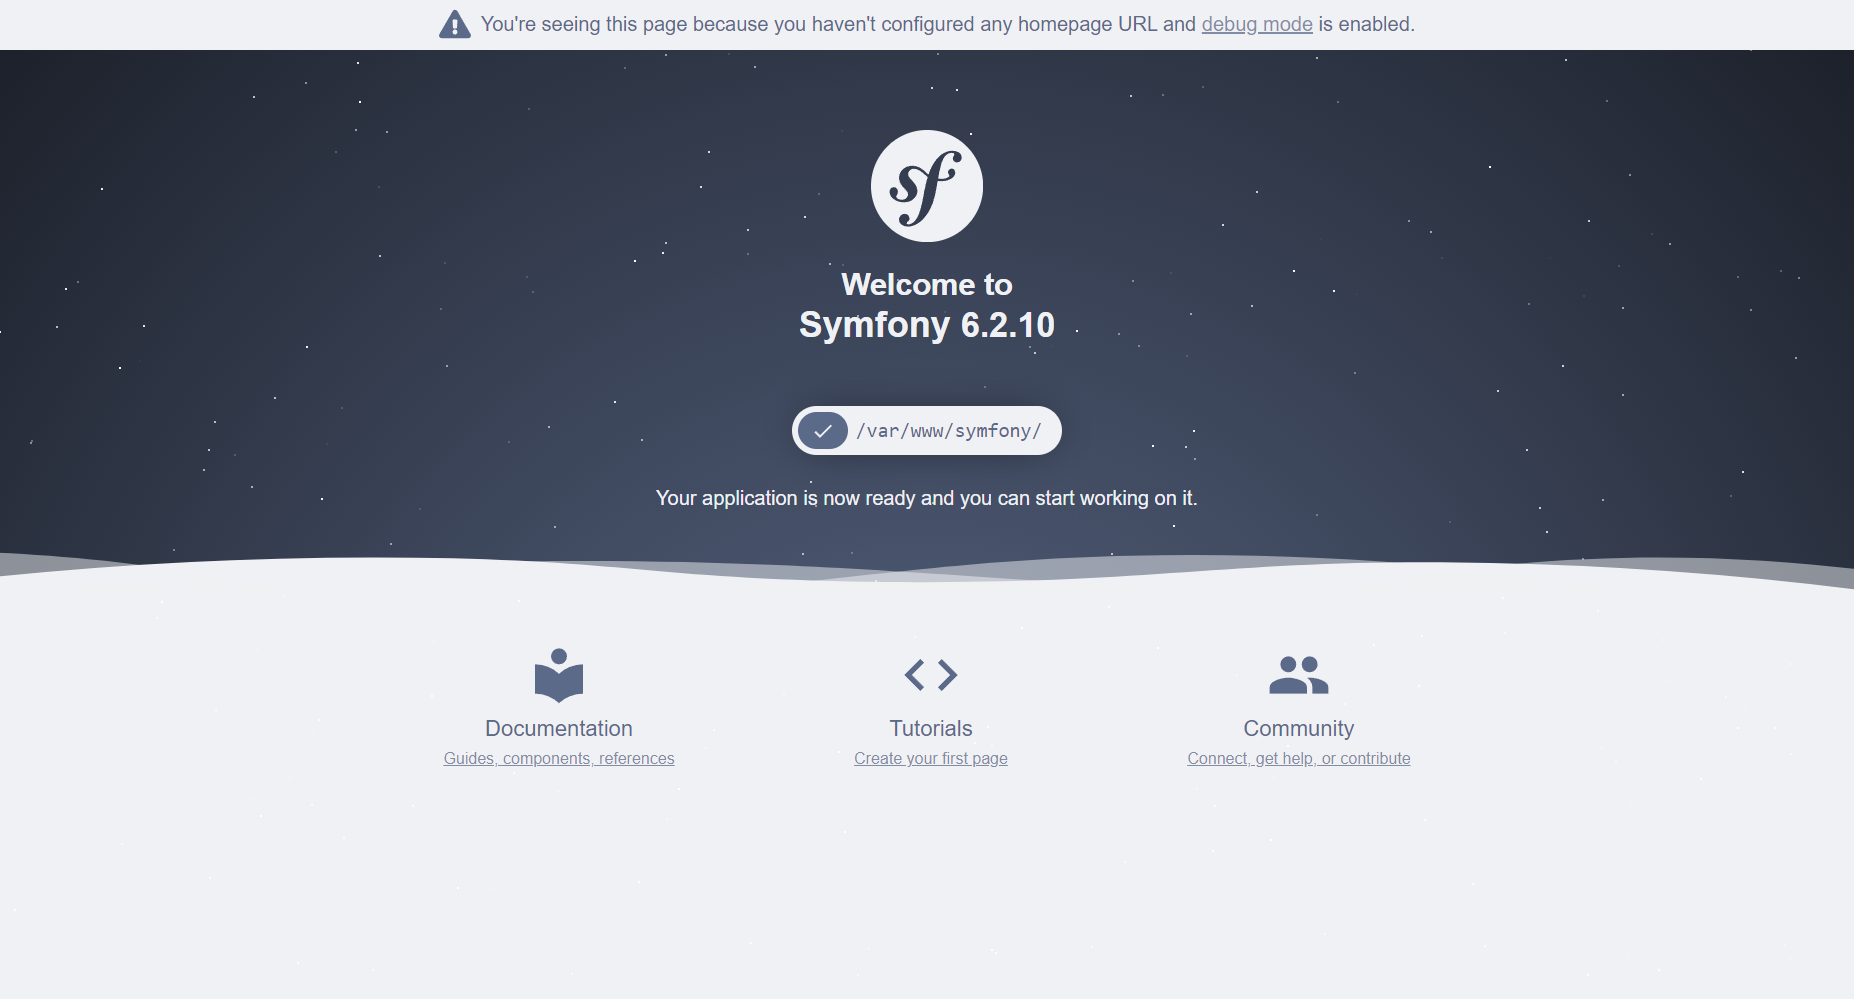
\includegraphics[width=\textwidth]{puste.png}
  \caption{Pusty projekt}
\end{figure}

\subsection{Struktura projektu}

Wejdźmy w kod za pomocą dowolnego edytora. Osobiście będę korzystał z PHPStorm. W katalogu \emph{src} znajduje się główna część kodu naszego projektu - obecnie jest niemalże pusta:

\begin{figure}[H]
  \centering
  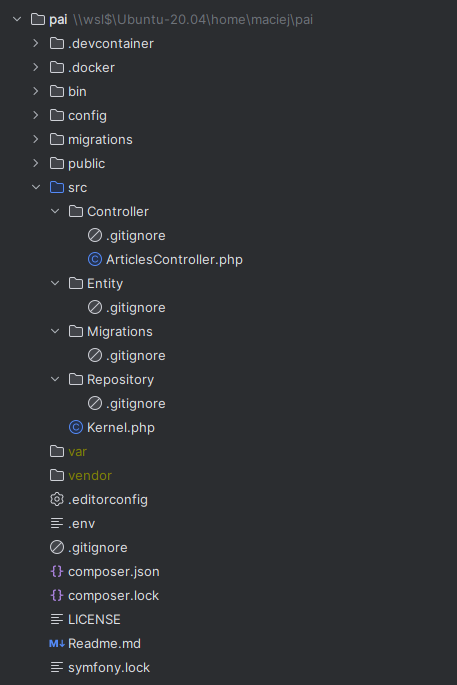
\includegraphics[width=0.4\textwidth]{struktura.png}
  \caption{Struktura projektu}
\end{figure}

Wejdźmy w plik \emph{Controller/ArticlesController.php} - to przykładowy kontroler dołączony w templatce:

\begin{lstlisting}[language=PHP, caption=Controller/ArticlesController.php]
<?php

namespace App\Controller;

use Symfony\Bundle\FrameworkBundle\Controller\AbstractController;
use Symfony\Component\HttpFoundation\Response;
use Symfony\Component\Routing\Annotation\Route;

class ArticlesController extends AbstractController
{
    #[Route(path: '/articles', name: 'articles', methods: ['GET'])]
    public function list(): Response
    {
        return new Response('Welcome to Latte and Code ');
    }
}
\end{lstlisting}

Możemy zauważyć, że nasz kontroler podłącza ścieżkę \emph{\\articles} pod kontroler \emph{ArticlesController->list()}, który zwraca odpowiedź tekstową. Sprawdźmy - wejdźmy w \emph{localhost/articles}:

\begin{figure}[H]
  \centering
  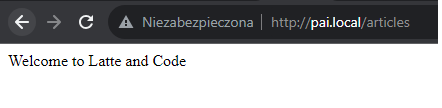
\includegraphics[width=\textwidth]{articles.png}
  \caption{Działa!}
\end{figure}

Fajnie, ale pisanie całego HTMLa w kontrolerze byłoby \emph{baaaardzo} uciążliwe. Wykorzystajmy więc Twiga!

\subsection{Twig (szablony) i recipes}

Twig to silnik szablonów dla języka programowania PHP. Jest to narzędzie często używane w połączeniu z frameworkiem Symfony, chociaż może być również stosowane samodzielnie. Twig zapewnia prosty i czytelny sposób definiowania szablonów, które są używane do generowania stron internetowych lub dowolnych innych treści tekstowych w PHP.

Wejdźmy w kontener PHP - wszystkie komendy związane z PHP uruchamiajmy zawsze wewnątrz kontenera! - i wykonajmy polecenie \emph{composer require template}.

Paczki zostaną automatycznie skonfigurowane:

\begin{verbatim}
Symfony operations: 2 recipes (561dabfd4bee7262baa401221aa62194)
  - Configuring symfony/twig-bundle (>=5.4): From github.com/symfony/recipes:main
  - Configuring twig/extra-bundle (>=v3.7.1): From auto-generated recipe
\end{verbatim}


\emph{auto-generated recipe} - co to? Już tłumaczę: Symfony Recipes to mechanizm, który automatyzuje proces konfigurowania paczek (bundles) oraz inne elementy w projekcie Symfony. 

\begin{description}

\item[Configuring symfony/twig-bundle (>=5.4): From github.com/symfony/recipes:main:]{
Symfony/twig-bundle to oficjalna paczka Symfony, która zapewnia integrację z Twig, silnikiem szablonów używanym w Symfony. W tej operacji, Symfony pobiera odpowiednią konfigurację dla paczki symfony/twig-bundle z repozytorium Symfony Recipes na GitHubie (github.com/symfony/recipes:main). Jest to centralne miejsce, w którym społeczność Symfony utrzymuje gotowe przepisy konfiguracyjne (Recipes) dla różnych paczek. Symfony automatycznie konfiguruje symfony/twig-bundle na podstawie przepisu znajdującego się w repozytorium.}

\end{description}

\textbf{W skrócie mówiąc, oszczędza nam to ręcznej konfiguracji :)}

Po wejściu w projekt możemy zauważyć, że pojawił się nowy katalog, a w nim jeden plik: \emph{templates/base.html.twig}. Paczka go automatycznie tworzyła - to będzie nasz bazowy motyw wykorzystywany dla każdej szablonowanej podstrony:

\begin{lstlisting}[caption=templates/base.html.twig]
<!DOCTYPE html>
<html>
    <head>
        <meta charset="UTF-8">
        <title>Welcome!</title>
        <link rel="icon" href="data:image/svg+xml,<svg xmlns=%22http://www.w3.org/2000/svg%22 viewBox=%220 0 128 128%22><text y=%221.2em%22 font-size=%2296%22></text></svg>">
        {# Run `composer require symfony/webpack-encore-bundle` to start using Symfony UX #}
        
            {{ encore_entry_link_tags('app') }}
        

        
            {{ encore_entry_script_tags('app') }}
        
    </head>
    <body>
        
    </body>
</html>
\end{lstlisting}

\subsection{Nasza pierwsza podstrona}

Chcemy stworzyć podstronę startową - utworzmy plik \emph{templates/index.html.twig}:

\begin{lstlisting}[caption=templates/index.html.twig]


Page Title


  <h1>Welcome to my website!</h1>
  <p>This is the content of the child template.</p>
  <p>Hello {{ hello }}!</p>

\end{lstlisting}

I załadujmy go w kontrolerze. Utwórzmy nowy kontroler, nazwijmy go \emph{IndexController.php}:

\begin{lstlisting}[language=PHP, caption=Controller/IndexController.php]
<?php

namespace App\Controller;

use Symfony\Bundle\FrameworkBundle\Controller\AbstractController;
use Symfony\Component\HttpFoundation\Response;
use Symfony\Component\Routing\Annotation\Route;

class IndexController extends AbstractController
{
    #[Route(path: '/', name: 'index', methods: ['GET'])]
    public function index(): Response
    {
        return $this->render('index.html.twig', [
            'hello' => 'World!'
        ]);
    }
}
\end{lstlisting}

Wejdźmy ponownie na \emph{localhost}:

\begin{figure}[H]
  \centering
  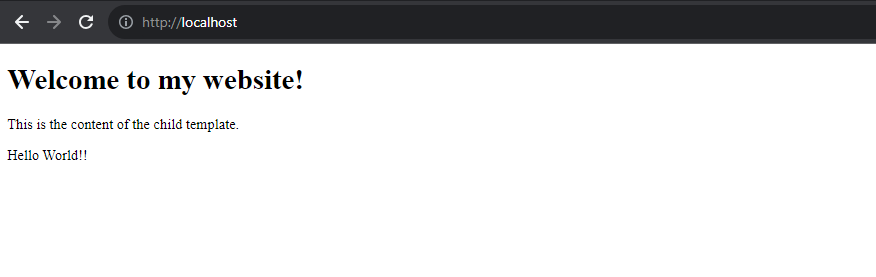
\includegraphics[width=\textwidth]{localhost hello.png}
  \caption{Działa - templatka została załadowana!}
\end{figure}

Po przeanalizowaniu kodu, możemy zauważyć że wykorzystaliśmy w Twigu bloki oraz zmienne, umożliwiając nam tworzenie rozszerzalnych templatek i przekazywanie danych z kontrolera do widoku.


\subsection{Poznajmy bundles}
Symfony posiada wiele paczek, które są nazywane \emph{bundle}. Bundles to moduły, które zawierają gotowe do użycia funkcje i komponenty, które można łatwo integrować z aplikacją Symfony. Te paczki ułatwiają development, ponieważ programiści nie muszą pisać wszystkiego od zera, ale mogą korzystać z gotowych rozwiązań, oszczędzając czas i wysiłek.

Bundles mogą zawierać różnorodne elementy, takie jak kontrolery, szablony widoków, konfiguracje, style CSS, skrypty JavaScript, a także specjalne funkcje, które rozszerzają możliwości frameworka Symfony. Dzięki nim programiści mogą szybko dodać funkcje do swoich aplikacji, takie jak uwierzytelnianie użytkowników, obsługa formularzy, integracja z bazą danych, obsługa plików multimedialnych i wiele innych.

\subsection{Wykorzystajmy bundles - użytkownicy}

W tym miejscu odwołam się do \href{https://symfony.com/doc/current/security.html}{oficjalnej dokumentacji Symfony pod tematem Security}, która również w tym miejscu świetnie przedstawia jak zrobić rzecz X w Symfony. Zgodnie z zaleceniami, wykorzystajmy security bundle:

Po uruchomieniu \emph{composer require symfony/security-bundle} możemy stworzyć użytkownika:

\begin{verbatim}
    php bin/console make:user
 The name of the security user class (e.g. User) [User]:
 > User

 Do you want to store user data in the database (via Doctrine)? (yes/no) [yes]:
 > yes

 Enter a property name that will be the unique "display" name for the user (e.g. email, username, uuid) [email]:
 > email

 Will this app need to hash/check user passwords? Choose No if passwords are not needed or will be checked/hashed by some other system (e.g. a single sign-on server).

 Does this app need to hash/check user passwords? (yes/no) [yes]:
 > yes

 created: src/Entity/User.php
 created: src/Repository/UserRepository.php
 updated: src/Entity/User.php
 updated: config/packages/security.yaml
\end{verbatim}

Skupmy się na tej części:

\begin{verbatim}
created: src/Entity/User.php
 created: src/Repository/UserRepository.php
 updated: src/Entity/User.php
 updated: config/packages/security.yaml
\end{verbatim}

Komenda utworzyła nam encję, która zostanie powiązana z tabelą bazodanową z wykorzystaniem Doctrine, czyli biblioteki ORM wykorzystywanej przez Symfony. Doctrine pozwala na definiowanie encji, relacji między encjami oraz operacji na danych za pomocą prostych metod PHP, co ułatwia manipulację danymi w bazie danych.

Encja to klasa PHP, która reprezentuje strukturę danych w bazie danych. Każda encja jest zwykle powiązana z określoną tabelą w bazie danych. Klasa encji definiuje pola (np. właściwości użytkownika, takie jak imię, email, itp.) oraz metody, które umożliwiają dostęp i manipulację tymi danymi. Doctrine, jako ORM, używa encji do mapowania danych między bazą danych a obiektami PHP, co ułatwia pracę z danymi w aplikacji.

Repozytorium to klasa, która zawiera logikę dostępu do danych związanych z daną encją. Repozytoria są używane do wykonywania zapytań do bazy danych, takich jak pobieranie, zapisywanie, aktualizowanie i usuwanie danych. Doctrine automatycznie generuje podstawowe repozytoria dla każdej encji, ale można je także dostosować, aby obsłużyć bardziej zaawansowane operacje na danych.

W kontekście Symfony, konfiguracja odnosi się do ustawień i parametrów aplikacji, które są zdefiniowane w różnych plikach konfiguracyjnych. W przypadku Doctrine, konfiguracja obejmuje informacje dotyczące połączenia z bazą danych, takie jak adres hosta, nazwa użytkownika, hasło, nazwa bazy danych, ale także konfiguracje związane z encjami i repozytoriami.

\subsection{Migracje - czyli stwórzmy schemat bazy danych}

Encja została stworzona, ale nie istnieje jeszcze w bazie danych. W tym celu musimy stworzyć i uruchomić migrację. 

Migracje bazodanowe to sposób zarządzania ewolucją schematu bazy danych w czasie, co oznacza, że możesz zmieniać strukturę bazy danych, dodając lub usuwając tabele, kolumny itp., w sposób kontrolowany i śledzony przez system kontroli wersji. Migracje pozwalają deweloperom na wprowadzanie zmian w schemacie bazy danych w sposób, który jest śledzony, dokumentowany i replikowalny na różnych środowiskach, takich jak lokalny komputer dewelopera, serwer testowy czy produkcji.

Wykonajmy następujące komendy:

\begin{itemize}
\item php bin/console make:migration
\item php bin/console doctrine:migrations:migrate
\end{itemize}

\begin{verbatim}
# bin/console ma:mi
  Success!

 Next: Review the new migration "migrations/Version20231015112242.php"
 Then: Run the migration with php bin/console doctrine:migrations:migrate
 See https://symfony.com/doc/current/bundles/DoctrineMigrationsBundle/index.html
# bin/console do:mi:mi

 WARNING! You are about to execute a migration in database "app_db" that could result in schema changes and data loss. Are you sure you wish to continue? (yes/no) [yes]:
 >

[notice] Migrating up to DoctrineMigrations\Version20231015112242
[notice] finished in 136.9ms, used 12M memory, 1 migrations executed, 1 sql queries

 [OK] Successfully migrated to version : DoctrineMigrations\Version20231015112242
\end{verbatim}

Po połączeniu się z bazą danych przez zewnętrzny klient możemy zauważyć, że powstała nasza pierwsza tabela:

\begin{figure}[H]
  \centering
  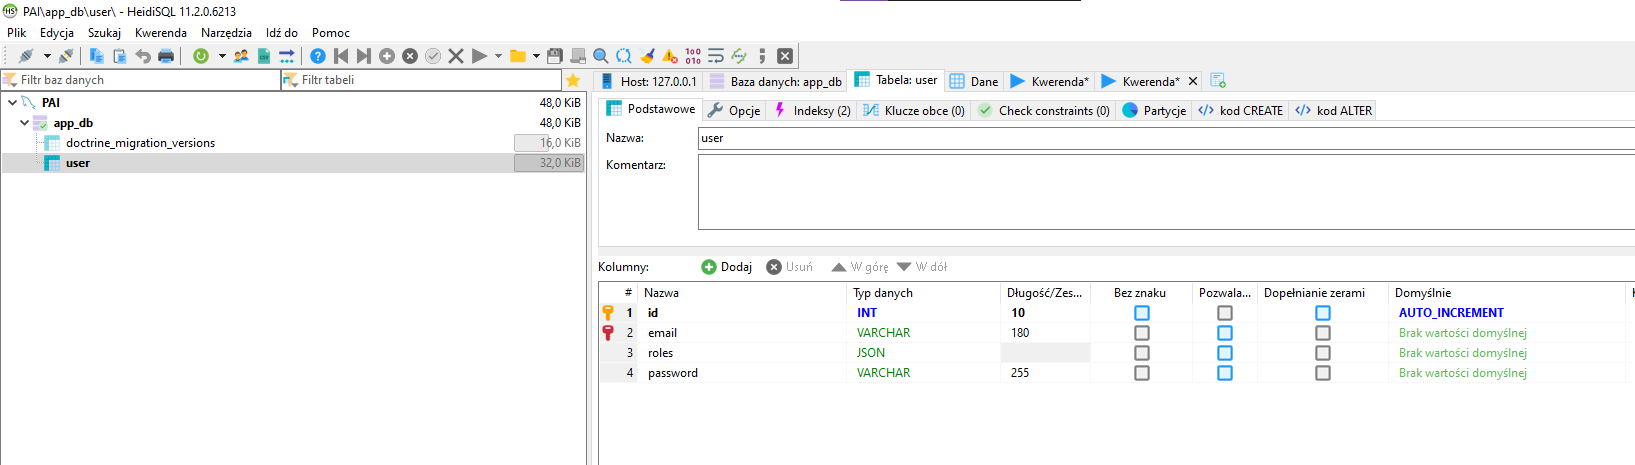
\includegraphics[width=\textwidth]{tabela.png}
  \caption{Działa!}
\end{figure}

Będziemy mogli zapisywać do bazy danych!

Stwórzmy nowego użytkownika. Obecnie skupmy się na samej czynności zapisywania, nie implementując formularza. Sprawmy, aby po wejściu na \emph{register} do bazy dodał się nowy użytkownik. Rozszerzmy nasz kontroler:

\begin{lstlisting}[language=PHP, caption=Controller/IndexController.php]
<?php

namespace App\Controller;

use App\Entity\User;
use Doctrine\ORM\EntityManagerInterface;
use Symfony\Bundle\FrameworkBundle\Controller\AbstractController;
use Symfony\Component\HttpFoundation\Response;
use Symfony\Component\PasswordHasher\Hasher\UserPasswordHasherInterface;
use Symfony\Component\Routing\Annotation\Route;

class IndexController extends AbstractController
{
    #[Route(path: '/', name: 'index', methods: ['GET'])]
    public function index(): Response
    {
        return $this->render('index.html.twig', [
            'hello' => 'World!'
        ]);
    }

    #[Route(path: '/register', name: 'register', methods: ['GET'])]
    public function register(
        UserPasswordHasherInterface $passwordHasher,
        EntityManagerInterface $entityManager,
    ): Response
    {
        $user = new User();
        $plaintextPassword = 'haslo';

        $user
            ->setEmail('test@example.com');

        $hashedPassword = $passwordHasher->hashPassword(
            $user,
            $plaintextPassword
        );
        $user->setPassword($hashedPassword);

        $entityManager->persist($user);
        $entityManager->flush();

        return new Response("Registered!");

    }
}
\end{lstlisting}

\subsection{Dependency Injection, Entity Manager - co to?}
Kluczowym punktem jest sposób, w jaki przekazywane są argumenty do metody register. Wielokrotne przekazywanie obiektów jako argumentów metod kontrolera jest przykładem techniki znaną jako Dependency Injection (DI).

Dependency Injection to wzorzec projektowy, który polega na przekazywaniu obiektów (zależności) do innych obiektów, zamiast pozwalania obiektom na samodzielne tworzenie ich zależności. W tym przypadku, metoda register przyjmuje dwie zależności: UserPasswordHasherInterface i EntityManagerInterface.

Dzięki temu podejściu, nie musisz ręcznie tworzyć obiektów tych zależności wewnątrz metody. Symfony automatycznie rozpoznaje typy zależności przekazane jako argumenty i dostarcza odpowiednie instancje tych typów podczas wywoływania metody.

Jak możemy zauważyć, w kodzie odwołujemy się również do EntityManagera w celu zapisania encji User. EntityManager to jedna z kluczowych części Doctrine, które jest narzędziem do mapowania obiektowo-relacyjnego (ORM), co oznacza, że pozwala programistom pracować z danymi w bazie danych, używając obiektów PHP, zamiast klasycznych zapytań SQL.

Doctrine wykorzystuje model Data Mapper zamiast Active Record, przez co zmiany nie naniosą się automatycznie, jak w Laravelu, tylko musimy wywołać persist() w celu oznaczenia obiektu jako nowego do zapisania, a następnie flush(), aby skomunikować się z bazą danych.

Wejdźmy na \emph{/register}:


\begin{figure}[H]
  \centering
  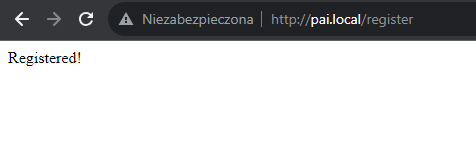
\includegraphics[width=\textwidth]{registered.png}
  \caption{Zarejestrowano - czy na pewno?}
\end{figure}

Komunikat pokazał, że zarejestrowano użytkownika. Czy na pewno? Podejrzyjmy w bazie danych:

\begin{figure}[H]
  \centering
  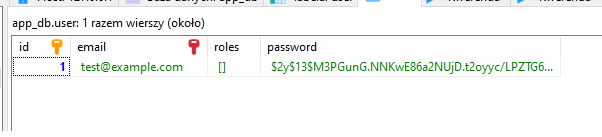
\includegraphics[width=\textwidth]{user.png}
  \caption{Zarejestrowano - na pewno :)}
\end{figure}

Udało się, zapisaliśmy pierwszego użytkownika w bazie danych. 

\subsection{Konfigurowanie encji i walidacja}
Spróbujmy wejść na podstronę ponownie:

\begin{figure}[H]
  \centering
  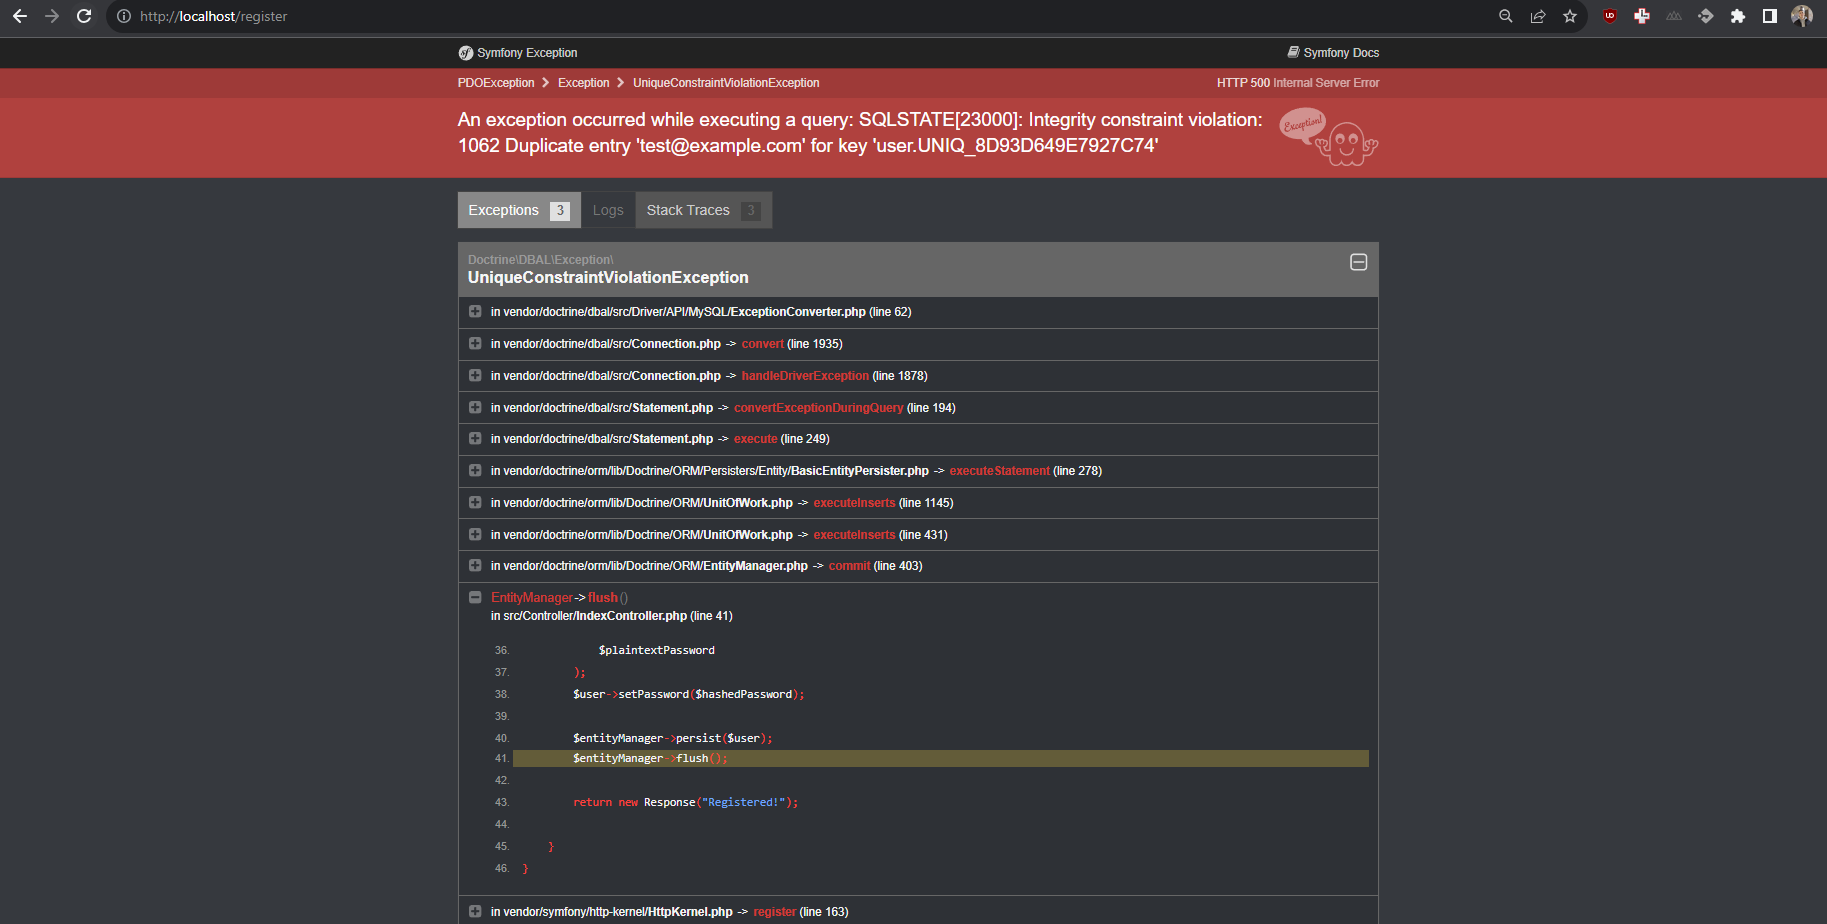
\includegraphics[width=\textwidth]{blad.png}
  \caption{Błąd?}
\end{figure}

Pojawił się błąd:

\begin{verbatim}
An exception occurred while executing a query: SQLSTATE[23000]: Integrity constraint violation: 
1062 Duplicate entry 'test@example.com' for key 'user.UNIQ_8D93D649E7927C74'
\end{verbatim}

Ten błąd oznacza, że próbujesz wstawić nowy rekord do tabeli w bazie danych, który narusza ograniczenie unikalności (unique constraint) na kolumnie o nazwie 'user.UNIQ\_8D93D649E7927C74'. W konkretnym przypadku, unikalność jest naruszona dla wartości 'test@example.com' w tej kolumnie. To oznacza, że w danej tabeli już istnieje rekord z wartością 'test@example.com', a próbujesz dodać kolejny rekord z tą samą wartością, co jest niedozwolone ze względu na ograniczenie unikalności.

Jak Symfony to wykryło? Wejdźmy do wcześniej utworzonej klasy \emph{src/Entity/User.php}:

\begin{lstlisting}[language=PHP, caption=src/Entity/User.php]
class User implements UserInterface, PasswordAuthenticatedUserInterface
{
    /* ... */
    
    #[ORM\Column(length: 180, unique: true)]
    private ?string $email = null;

    /* ... */
\end{lstlisting}

Atrybut \emph{ORM\\Column} określa nam, że kolumna powinna mieć maksymalnie 180 znaków, powinna być unikalna, zaś typ jest odczytywany z typu zmiennej. Na tej podstawie generowany jest kod SQL, który tworzy nam schema w bazie danych! 

Założenie jest poprawne. Zmodyfikujmy więc nasz kontroler, aby dodać drugiego użytkownika:

\begin{lstlisting}[language=PHP, caption=Controller/IndexController.php]
        $user
            ->setEmail('to nie jest email!!!11');
\end{lstlisting}

I wejdźmy na /register ponownie:

\begin{figure}[H]
  \centering
  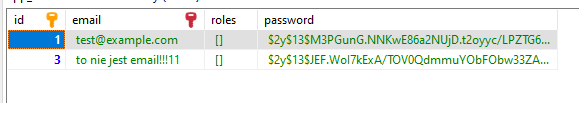
\includegraphics[width=\textwidth]{email2.png}
  \caption{Halo, to nielegalne!}
\end{figure}

Chwila - przecież powinniśmy móc dodawać tylko email! Dodajmy walidację. Zainstalujmy komponent odpowiadający za walidację: \emph{composer require symfony/validator}

Po instalacji możemy dodać nasz pierwszy constraint:

\begin{lstlisting}[language=PHP, caption=Entity/User.php]
use Symfony\Component\Validator\Constraints as Assert;

class User implements UserInterface, PasswordAuthenticatedUserInterface
{
    #[ORM\Column(length: 180, unique: true)]
    #[Assert\Email(
        message: 'Dobrodzieju, podana przez Wacpana wartosc {{ value }} nie jest poprawnym adresem poczty elektronicznej!',
    )]
    private ?string $email = null;
\end{lstlisting}

Spróbujmy ponownie dodać użytkownika z niepoprawnym adresem email. Po uruchomieniu /register... nic się nie stanie! Dlaczego? Ponieważ musimy jeszcze wywołać walidację. Przy formularzach walidacja uruchamiana jest automatycznie, co oszczędza nam roboty, ale tutaj pokazujemy mechanizm od podstaw :)

\begin{lstlisting}[language=PHP, caption=Controller/IndexController.php]
    #[Route(path: '/register', name: 'register', methods: ['GET'])]
    public function register(
        UserPasswordHasherInterface $passwordHasher,
        EntityManagerInterface $entityManager,
        ValidatorInterface $validator,
    ): Response
    {
        $user = new User();
        $plaintextPassword = 'haslo';

        $user
            ->setEmail('to nie jest email!!!11');

        $hashedPassword = $passwordHasher->hashPassword(
            $user,
            $plaintextPassword
        );
        $user->setPassword($hashedPassword);

        $errors = $validator->validate($user);

        if (count($errors) > 0) {
            $errorMessages = [];
            foreach ($errors as $error) {
                $errorMessages[$error->getPropertyPath()] = $error->getMessage();
            }

            return new Response(implode("<br>", $errorMessages), Response::HTTP_BAD_REQUEST);
        }

        $entityManager->persist($user);
        $entityManager->flush();

        return new Response("Registered!");

    }
\end{lstlisting} 

W przypadku wystąpienia błędów z walidatora, pojawi się komunikat na ekranie, a użytkownik nie zostanie zapisany:


\begin{figure}[H]
  \centering
  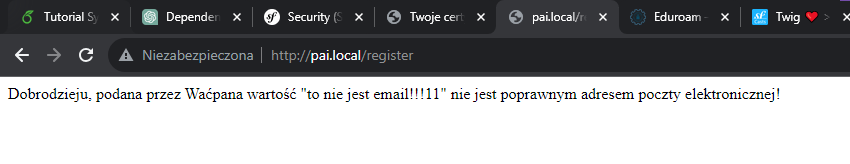
\includegraphics[width=\textwidth]{wacpan.png}
  \caption{Waćpanie, tak nie można!}
\end{figure}

Działa! Symfony posiada \href{https://symfony.com/doc/current/validation.html}{wiele wbudowanych walidatorów}:

\begin{figure}[H]
  \centering
  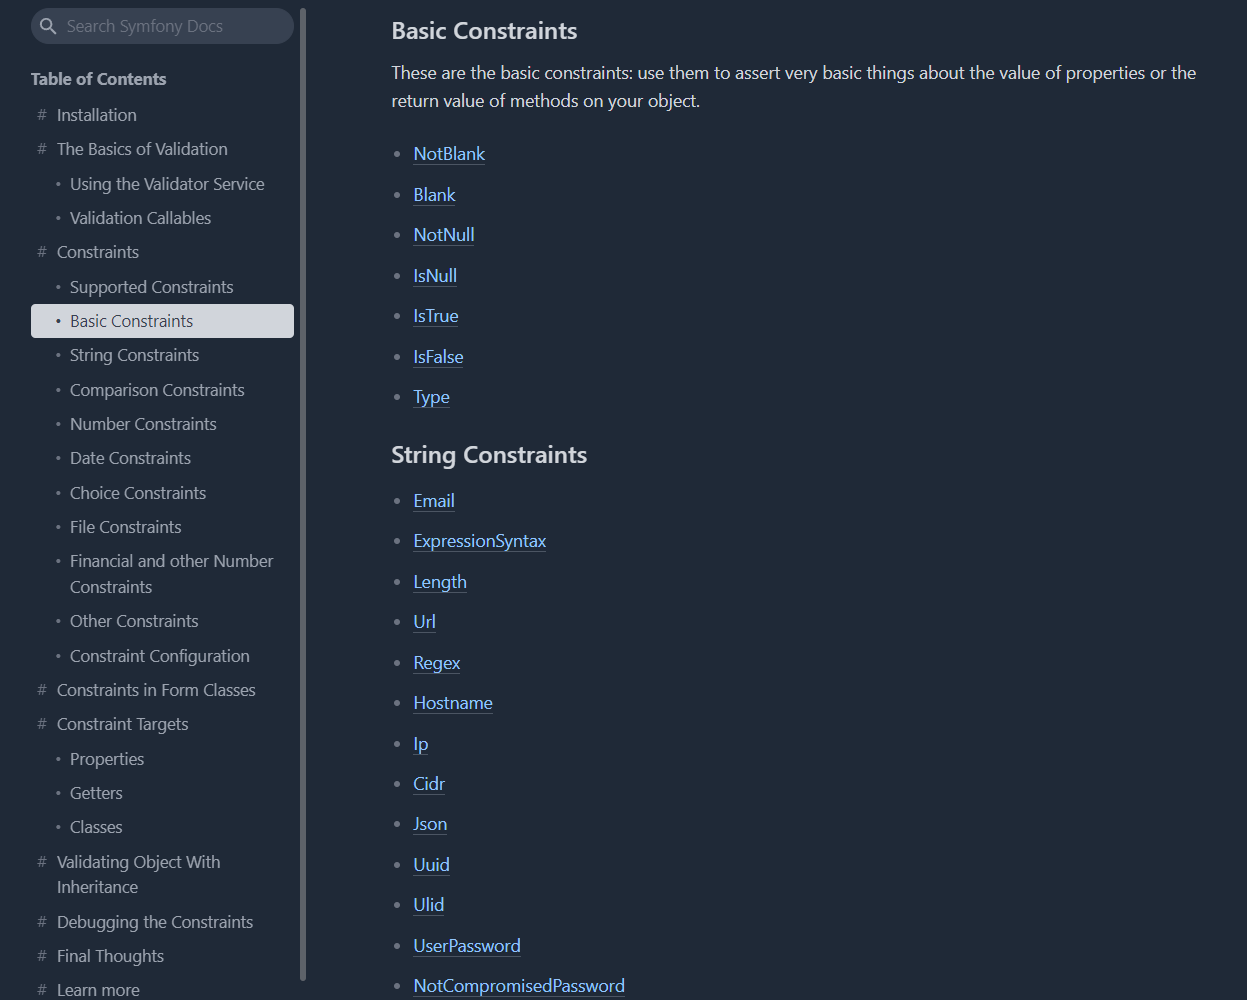
\includegraphics[width=\textwidth]{walidacja.png}
  \caption{Walidacja - zrzut ekranu oficjalnej dokumentacji}
\end{figure}

Jak widać, jest ich naprawdę multum.

\subsection{Debugging w Symfony - Profiler}

Symfony jest świetne pod kątem debuggingu. Jak widać na poprzednim zrzucie ekranu, przy błędzie pojawia się duży, czerwony stacktrace. Dodajmy gdzieś exception: \emph{throw new \\Exception("Blad. Skad on sie wzial?");}

\begin{figure}[H]
  \centering
  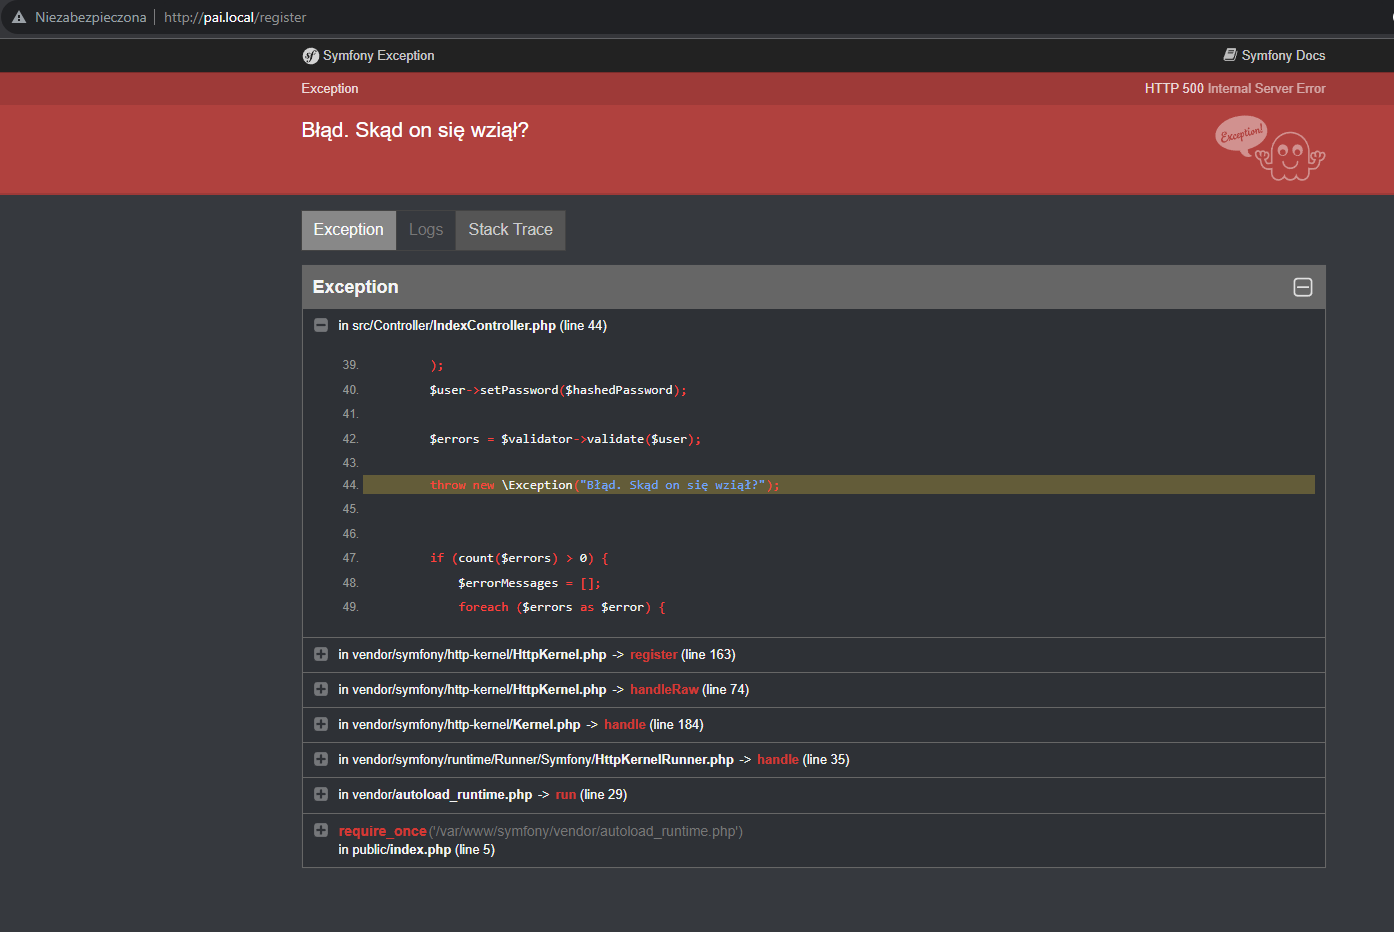
\includegraphics[width=\textwidth]{blad2.png}
  \caption{Błąd}
\end{figure}

Dlaczego Symfony jest świetne? Zainstalujmy paczkę aby się dowiedzieć: \emph{composer require --dev symfony/profiler-pack}.

Po zainstalowaniu możemy zauważyć, że pojawił się na dole czarny pasek:

\begin{figure}[H]
  \centering
  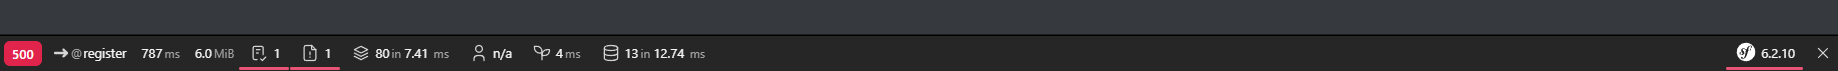
\includegraphics[width=\textwidth]{profiler.png}
  \caption{Czarny pasek na dole ekranu - Profiler}
\end{figure}

Kliknijmy w lewy dolny róg, a pojawi się pełen ekran Profilera:

\begin{figure}[H]
  \centering
  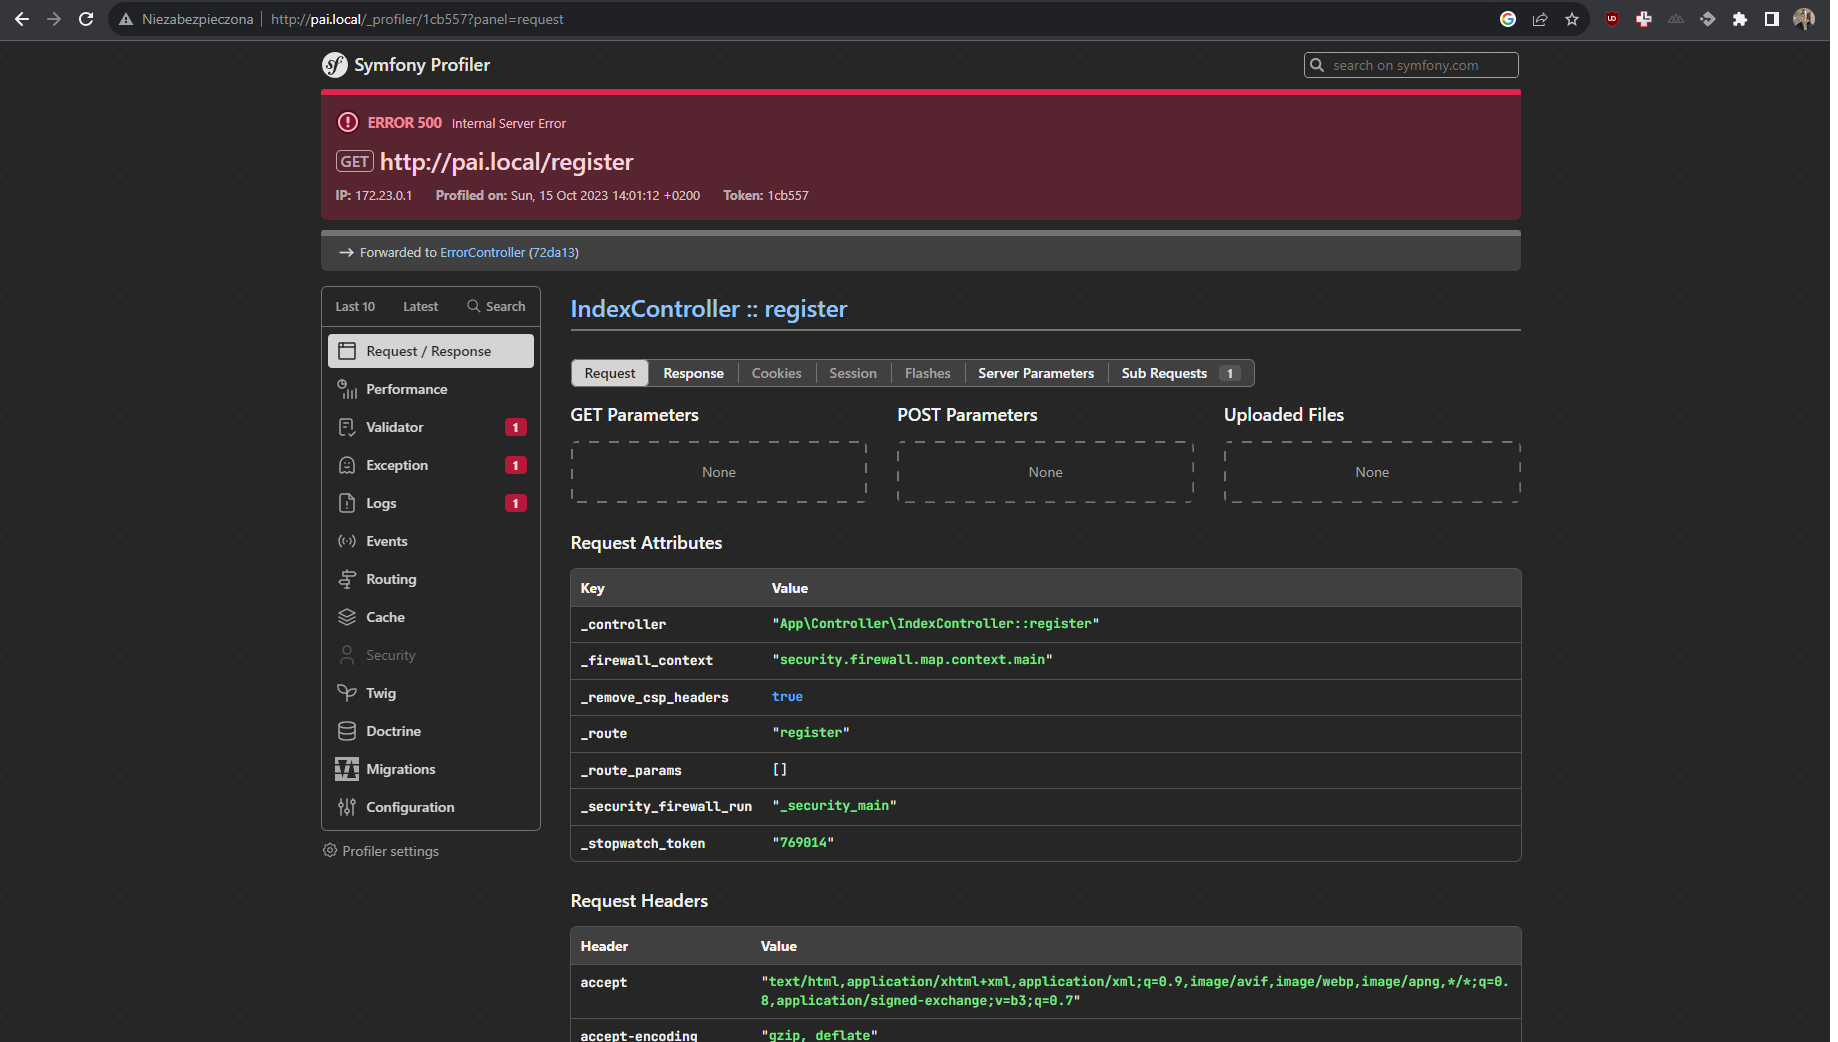
\includegraphics[width=\textwidth]{profiler2.png}
  \caption{Profiler}
\end{figure}

Profiler pozwala na śledzenie żądań HTTP, analizę wydajności, monitorowanie zapytań SQL, śledzenie błędów i wyjątków, przeglądanie logów aplikacji oraz sprawdzanie, które fragmenty kodu zajmują najwięcej czasu wykonania. Dzięki Profilerowi deweloperzy mogą precyzyjnie zlokalizować i zrozumieć problemy w aplikacji, ułatwiając szybkie debugowanie, optymalizację kodu oraz eliminowanie błędów.

Wejdźmy przykładowo w zakładkę \emph{Validator}:

\begin{figure}[H]
  \centering
  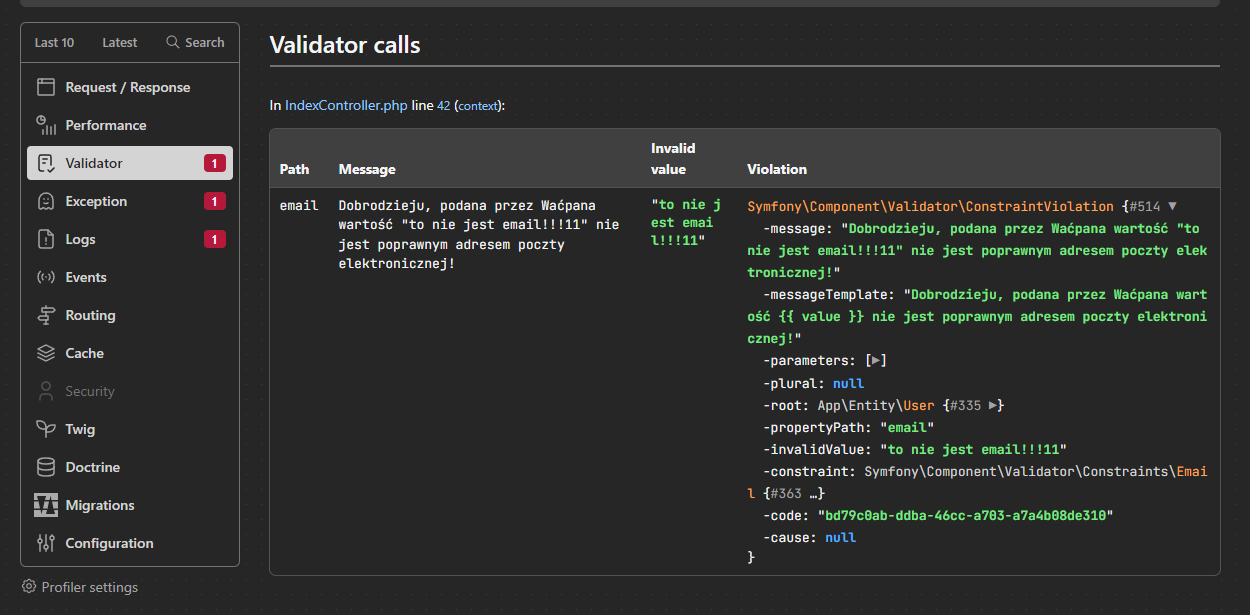
\includegraphics[width=\textwidth]{validator.png}
  \caption{Sekcja Validator w Profilerze}
\end{figure}

Informacje w Profilerze pojawią się zawsze. Sam Profiler można wyłączyć na środowisku uat/prod za pomocą zmiennych środowiskowych.

\subsection{Formularze - potęga Symfony}

Zaletą silnego systemu formularzy w Symfony jest jego intuicyjny i rozbudowany mechanizm, który pozwala programistom łatwo tworzyć, walidować i przetwarzać formularze. Framework automatyzuje wiele kroków, takich jak generowanie kodu HTML, obsługa walidacji danych, zarządzanie błędami i przetwarzanie danych wejściowych od użytkownika. Dzięki temu, programiści mogą efektywnie budować interaktywne interfejsy użytkownika, skupiając się na logice aplikacji, a nie na szczegółach obsługi formularzy, co przyspiesza rozwój aplikacji i poprawia jakość kodu.

Stwórzmy nasz pierwszy formularz. Zainstalujmy paczkę: \emph{composer require form}

W tym miejscu stwórzmy dodatkową encję - nazwijmy ją Zawody (SportsEvent). Nie będziemy w tutorialu przedstawiali operowania na encji User, ponieważ nie pokaże nam to zalet operowania na Symfony.

Do tworzenia encji wykorzystajmy Maker Bundle. Maker Bundle to już zainstalowana paczka, która ułatwia pisanie kodu:

\begin{verbatim}
make
  make:auth                                  Creates a Guard authenticator of different flavors
  make:command                               Creates a new console command class
  make:controller                            Creates a new controller class
  make:crud                                  Creates CRUD for Doctrine entity class
  make:docker:database                       Adds a database container to your docker-compose.yaml file
  make:entity                                Creates or updates a Doctrine entity class, and optionally an API Platform resource
  make:fixtures                              Creates a new class to load Doctrine fixtures
  make:form                                  Creates a new form class
  make:message                               Creates a new message and handler
  make:messenger-middleware                  Creates a new messenger middleware
  make:migration                             Creates a new migration based on database changes
  make:registration-form                     Creates a new registration form system
  make:reset-password                        Create controller, entity, and repositories for use with symfonycasts/reset-password-bundle
  make:serializer:encoder                    Creates a new serializer encoder class
  make:serializer:normalizer                 Creates a new serializer normalizer class
  make:stimulus-controller                   Creates a new Stimulus controller
  make:subscriber                            Creates a new event subscriber class
  make:test                                  [make:unit-test|make:functional-test] Creates a new test class
  make:twig-component                        Creates a twig (or live) component
  make:twig-extension                        Creates a new Twig extension with its runtime class
  make:user                                  Creates a new security user class
  make:validator                             Creates a new validator and constraint class
  make:voter                                 Creates a new security voter class
\end{verbatim}

My wykorzystamy komendę \emph{bin/console make:entity}:

\begin{verbatim}
# bin/console make:entity

 Class name of the entity to create or update (e.g. AgreeablePuppy):
 > SportsEvent
 created: src/Entity/SportsEvent.php
 created: src/Repository/SportsEventRepository.php

 Entity generated! Now let's add some fields!
 You can always add more fields later manually or by re-running this command.

 New property name (press <return> to stop adding fields):
 > name
 Field type (enter ? to see all types) [string]:
 >
 Field length [255]:
 >

 Can this field be null in the database (nullable) (yes/no) [no]:
 >
 updated: src/Entity/SportsEvent.php

 Add another property? Enter the property name (or press <return> to stop adding fields):
 > date
 Field type (enter ? to see all types) [string]:
 > datetime
 Can this field be null in the database (nullable) (yes/no) [no]:
 >
 updated: src/Entity/SportsEvent.php

 Add another property? Enter the property name (or press <return> to stop adding fields):
 >
  Success!
 Next: When you're ready, create a migration with php bin/console make:migration

#
\end{verbatim}

Powinna utworzyć nam się encja \emph{SportsEvent}. Stwórzmy i wykonajmy migrację:

\begin{verbatim}
# bin/console ma:mi

  Success!

 Next: Review the new migration "migrations/Version20231015121816.php"
 Then: Run the migration with php bin/console doctrine:migrations:migrate
 See https://symfony.com/doc/current/bundles/DoctrineMigrationsBundle/index.html
# bin/console do:mi:mi

 WARNING! You are about to execute a migration in database "app_db" that could result in schema changes and data loss. Are you sure you wish to continue? (yes/no) [yes]:
 >

[notice] Migrating up to DoctrineMigrations\Version20231015121816
[notice] finished in 143.5ms, used 16M memory, 1 migrations executed, 1 sql queries

 [OK] Successfully migrated to version : DoctrineMigrations\Version20231015121816

#
\end{verbatim}

Baza została zaktualizowana, utworzyliśmy encję SportsEvent z nazwą i datą. Utwórzmy dla niej formularz:

\begin{verbatim}
# bin/console make:form

 The name of the form class (e.g. GentlePizzaType):
 > SportsEventType

 The name of Entity or fully qualified model class name that the new form will be bound to (empty for none):
 > SportsEvent

 created: src/Form/SportsEventType.php

  Success!

 Next: Add fields to your form and start using it.
 Find the documentation at https://symfony.com/doc/current/forms.html
#
\end{verbatim}

Pojawił się nowy plik - \emph{Form/SportsEventType.php}:

\begin{lstlisting}[language=PHP, caption=Form/SportsEventType.php]
<?php

namespace App\Form;

use App\Entity\SportsEvent;
use Symfony\Component\Form\AbstractType;
use Symfony\Component\Form\FormBuilderInterface;
use Symfony\Component\OptionsResolver\OptionsResolver;

class SportsEventType extends AbstractType
{
    public function buildForm(FormBuilderInterface $builder, array $options): void
    {
        $builder
            ->add('name')
            ->add('date')
        ;
    }
    public function configureOptions(OptionsResolver $resolver): void
    {
        $resolver->setDefaults([
            'data_class' => SportsEvent::class,
        ]);
    }
}
\end{lstlisting}

Wyświetlmy nasz formularz, tworząc nowy kontroler:
\begin{lstlisting}[language=PHP]
    #[Route(path: '/form', name: 'form', methods: ['GET', 'POST'])]
    public function form(Request $request, EntityManagerInterface $entityManager): Response
    {
        $sportsEvent = new SportsEvent();

        $form = $this->createForm(SportsEventType::class, $sportsEvent);

        $form->handleRequest($request);

        if ($form->isSubmitted() && $form->isValid()) {
            $entityManager->persist($sportsEvent);
            $entityManager->flush();
            return $this->redirectToRoute('index');
        }

        return $this->render('form.html.twig', [
            'form' => $form->createView(),
        ]);
    }
\end{lstlisting}

Utwórzmy też plik \emph{form.html.twig}:

\begin{lstlisting}


Formularz


  {{ form(form) }}

\end{lstlisting}

I wejdźmy na \emph{/form}:

\begin{figure}[H]
  \centering
  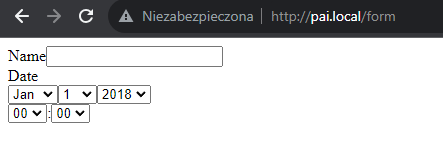
\includegraphics[width=\textwidth]{form.png}
  \caption{Formularz jest widoczny!}
\end{figure}

Pojawił się formularz! Kod w kontrolerze wspiera wysyłkę, jednak nie możemy go wysłać po stronie przeglądarki. Dodajmy do formularza jeszcze pole typu \emph{SubmitType}, które umożliwi wysyłkę.

\begin{lstlisting}[language=PHP]
use Symfony\Component\Form\Extension\Core\Type\SubmitType;

class SportsEventType extends AbstractType
{
    public function buildForm(FormBuilderInterface $builder, array $options): void
    {
        $builder
            ->add('name')
            ->add('date')
            ->add('submit', SubmitType::class, [
                'label' => 'Submit',
            ])
        ;
    }
\end{lstlisting}

Odświeżmy stronę:

\begin{figure}[H]
  \centering
  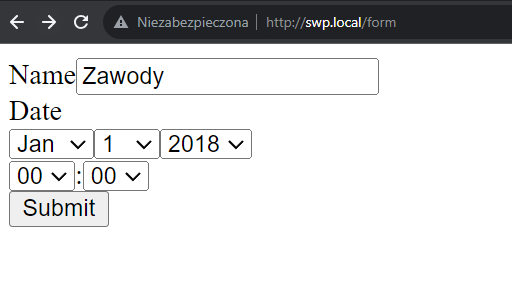
\includegraphics[width=\textwidth]{submit.png}
  \caption{Pojawił się przycisk Submit}
\end{figure}

Super - spróbujmy wypełnić formularz. Po naciśnięciu Submit zaobserwujemy przekierowanie na stronę główną, a po wejściu do bazy danych:

\begin{figure}[H]
  \centering
  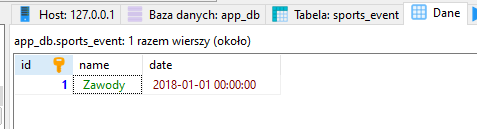
\includegraphics[width=\textwidth]{zawody.png}
  \caption{Działa - zawody zostały zapisane w bazie!}
\end{figure}

Wszystko działa - za pomocą niewielkiej ilości kodu udało nam się stworzyć formularz zapisujący do bazy!

\section{Odnośniki}

\begin{description}
    \item[Kod dla powyższego poradnika razem z chronologiczną historią commitów]{\href{https://github.com/mkaszkowiak-cs-put/podstawy-aplikacji-internetowych}{https://github.com/mkaszkowiak-cs-put/podstawy-aplikacji-internetowych}}
    \item[Oficjalna dokumentacja Symfony, obszerna, zrozumiała oraz aktualna]{\href{https://symfony.com/}{https://symfony.com/}}
    \item[SymfonyCasts, nieoficjalna dokumentacja, świetnie pokazuje przykłady]{\href{https://symfonycasts.com/screencast/symfony5/twig-recipe}{https://symfonycasts.com/screencast/symfony5/twig-recipe}}
\end{description}

\section{O dokumencie}

\textbf{Niniejszy dokument może być redystrybuowany i modyfikowany bez zgody autora.} Drobny disclaimer - autor pisał na szybko i dokument może zawierać błędy stylistyczne ;) 

\end{document}


